\section{Results and Discussion}

This section contains our main results and the discussion. First, we present our \co prediction, which is the output from our trained sector models. Afterwards, we dig deeper into our data, and reveal, which sectors were de- or increasing the most. The second part is dedicated to the analysis of the COVID-19 impact, where we briefly analyze the developments so far, and correlate different metrics in a time series fashion and a simpler integrated correlation plot. The third part relates those correlations with the goals of the paris climate agreement. Finally, we conclude the section with a thorough discussion of the validity of our data and an answer to the research question.

\subsection*{\co emission drop in all countries}

We start with presenting the main result of our sector resolved \co prediction approach. In Figure \ref{fig:expected_change_rate}, the predicted change rates per month and country are illustrated.

\begin{figure}[H]
	\centering
	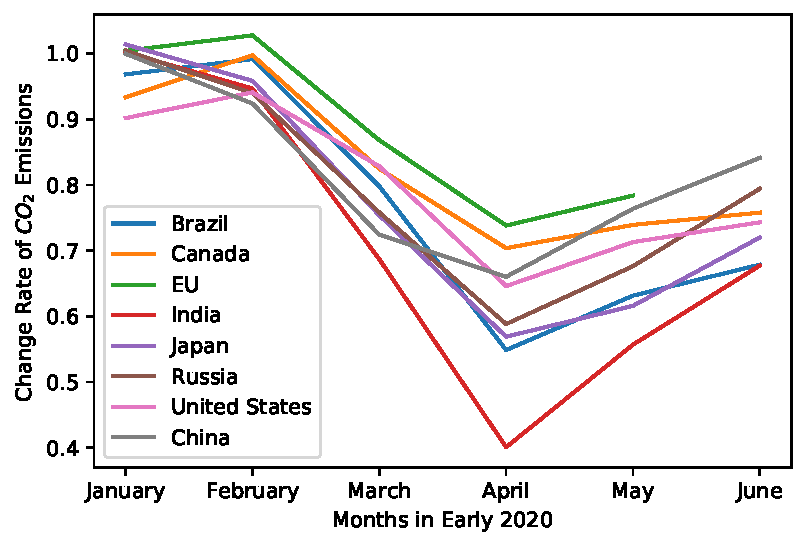
\includegraphics[width=0.7\textwidth]{img/change_rate.pdf}
	\caption{Overall expected change rate.}
	\label{fig:expected_change_rate}
\end{figure}

Here we can observe that the emissions were more or less the same during January and February, just before the beginning of the corona crisis. Then, from March on, when countries followed Chinas lock down approach with their own policies, we can see a clear drop in emissions, resulting in a \co emission performance between 0.8 and 0.4. From May on, the lock-down phase was abolished in many countries. This explains that the emissions start climbing again to a pre-COVID-19 regime.

In summary, the relative emission drop was most prominent in India (down to 40\%), whereas the EU, Canada, USA and China showed a more robust response of minimum emission values around 70\%.

In fact, COVID-19 impacted India's economy probably more severely then others. According to an article published by Maurice Kugler and Shakti Sinha in July 2020, 400 million people risk falling into poverty due to COVID-19 \cite{Kugler}, which is not only a significantly larger fraction of the population than in any other country, but also a more substantial threat than temporal unemployment.

\subsection*{Sector trends: Power industry as the leading sector}%todo: Pie charts

But what led to the decrease of emissions in the first place? We try to approach this question, by analyzing the individual performance of single sectors in each country. For the different plots in Figures \ref{fig:bar_plots} and \ref{fig:bar_plots2}, the performance vectors where averaged over the period of the year 2020 so far.

\begin{figure}[H]
	\centering
	\subfloat[Brazil]{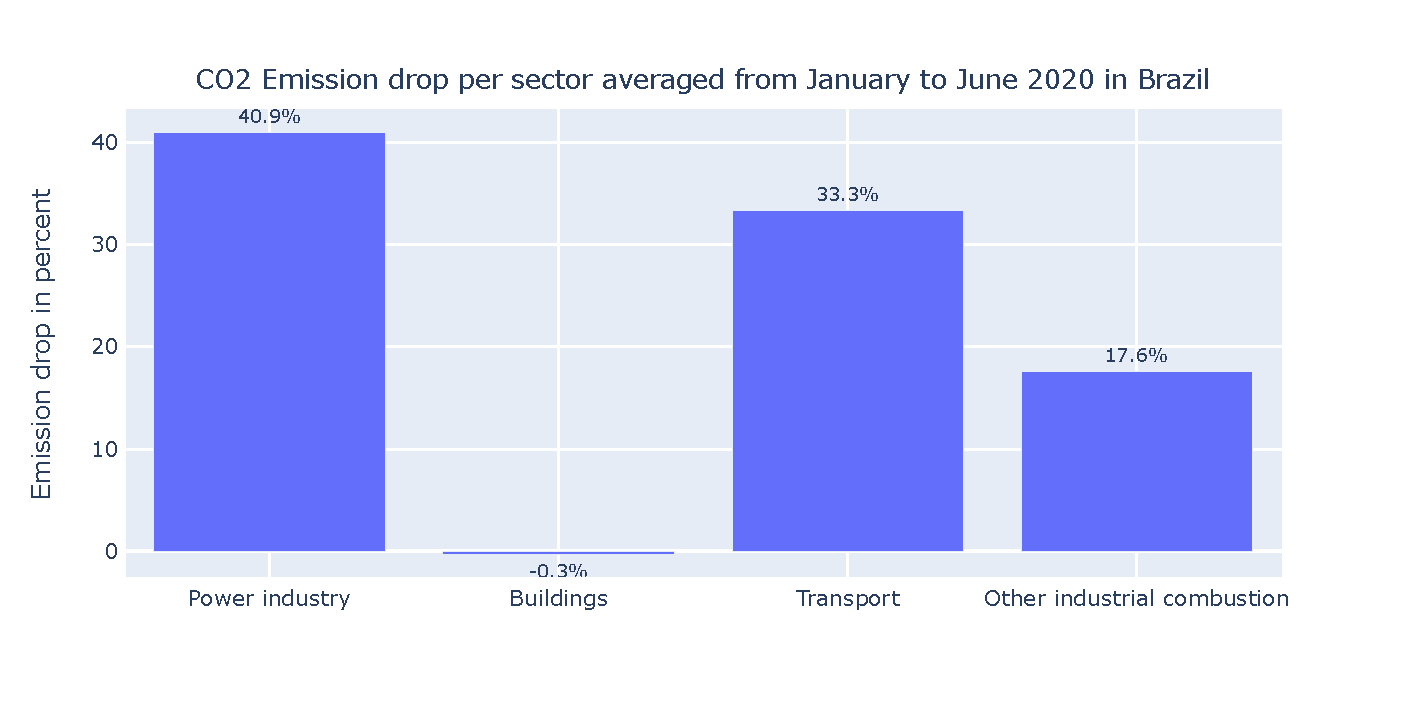
\includegraphics[width=0.45\linewidth]{../sector_overview/bar_plot_Brazil}}
	\subfloat[Brazil]{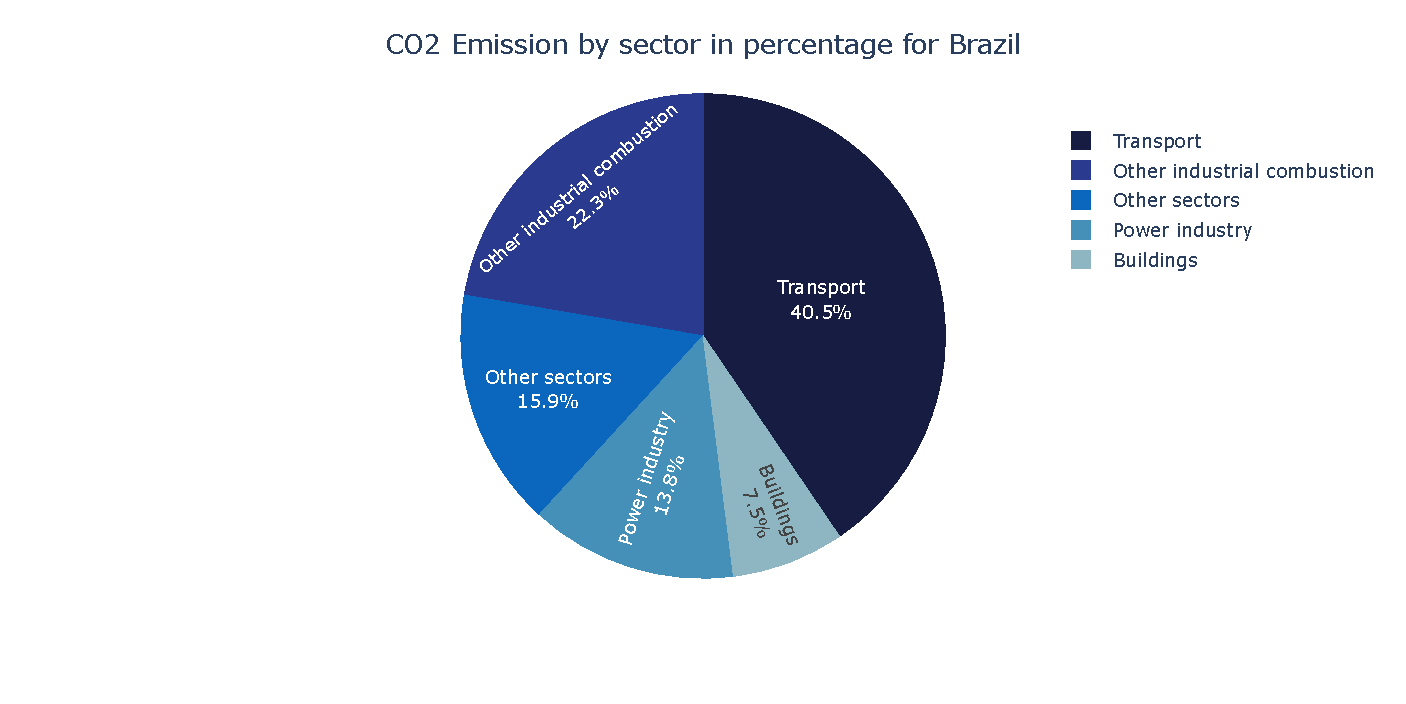
\includegraphics[width=0.45\linewidth]{../sector_overview/pie_plot_Brazil}}\\
	\subfloat[Canada]{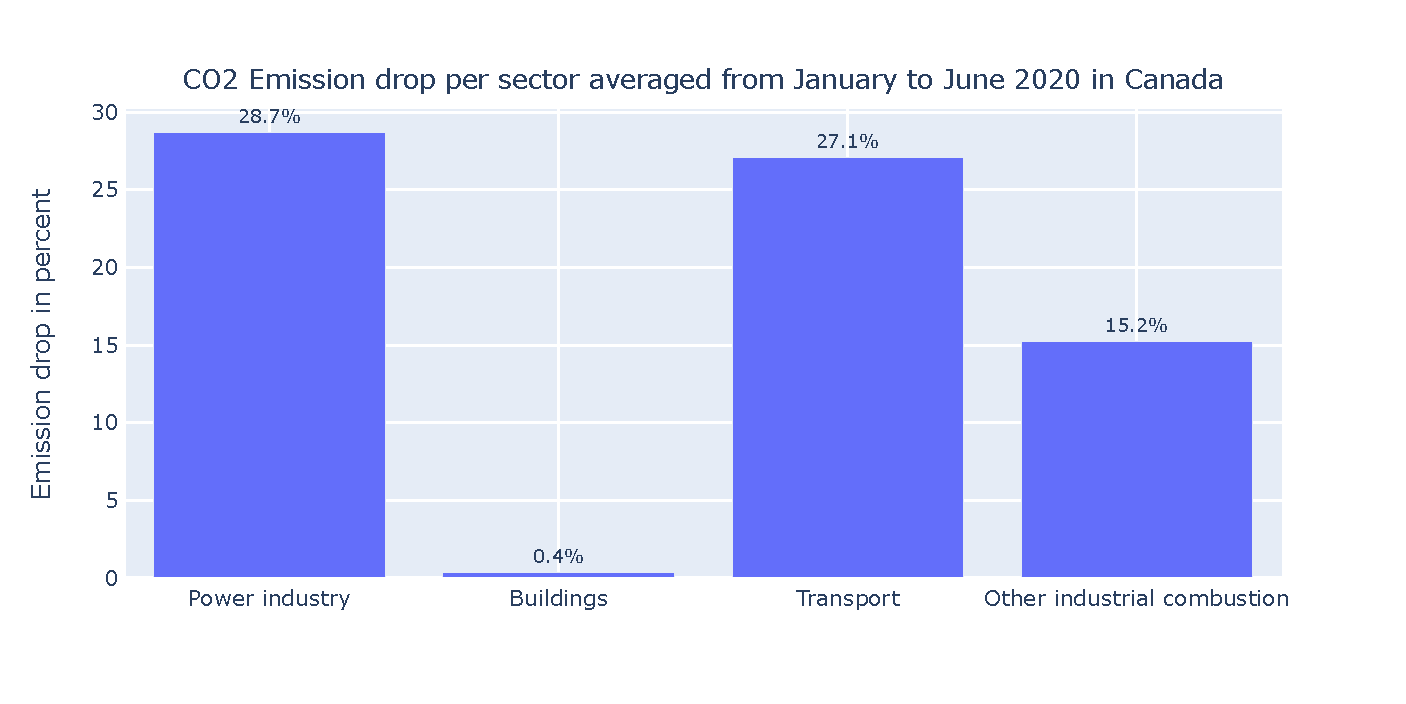
\includegraphics[width=0.45\linewidth]{../sector_overview/bar_plot_Canada}}
	\subfloat[Canada]{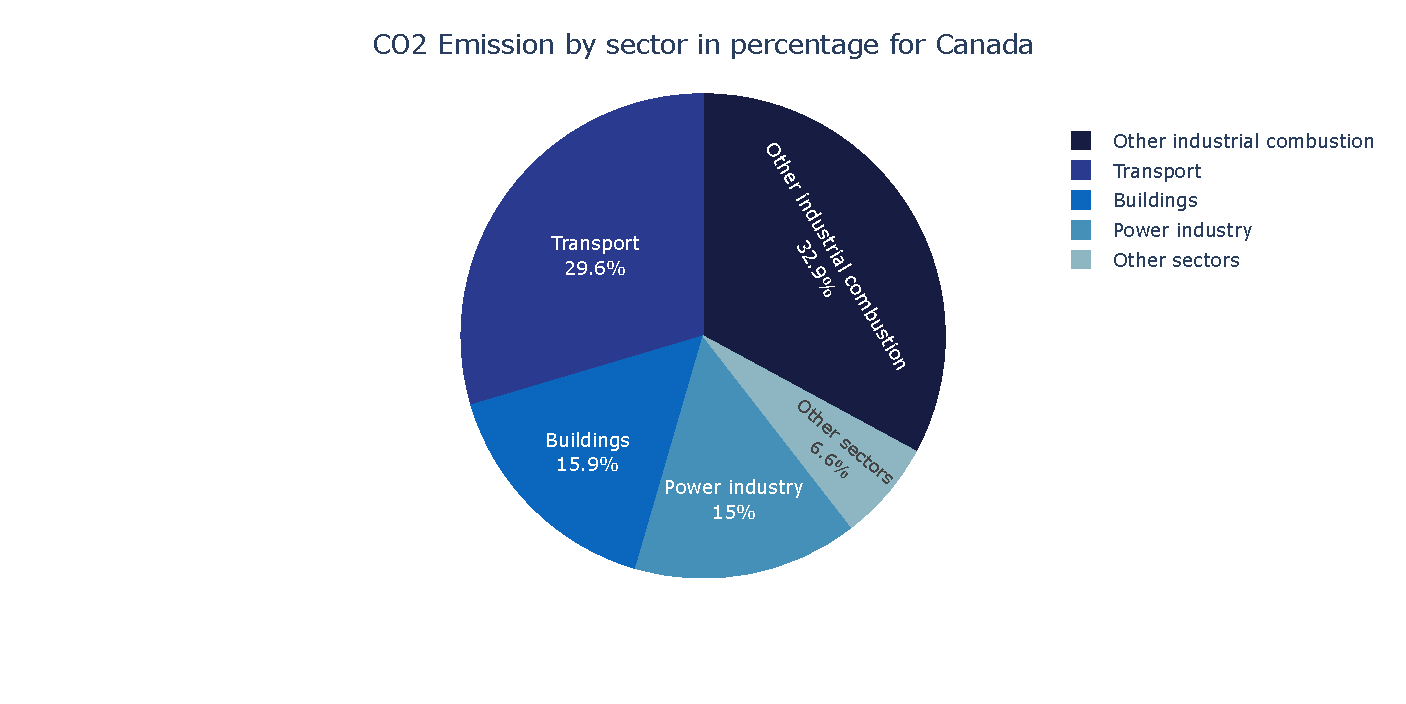
\includegraphics[width=0.45\linewidth]{../sector_overview/pie_plot_Canada}}\\
	\subfloat[China]{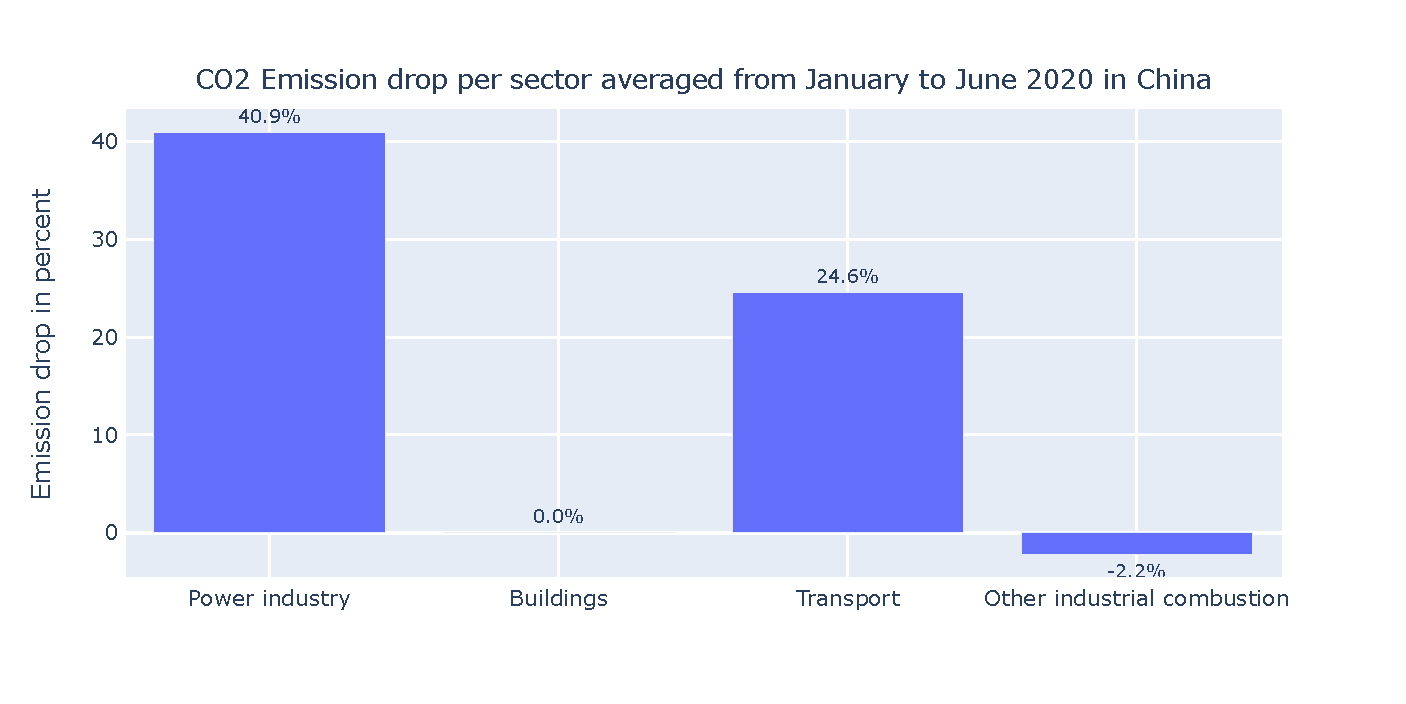
\includegraphics[width=0.45\linewidth]{../sector_overview/bar_plot_China}}
	\subfloat[China]{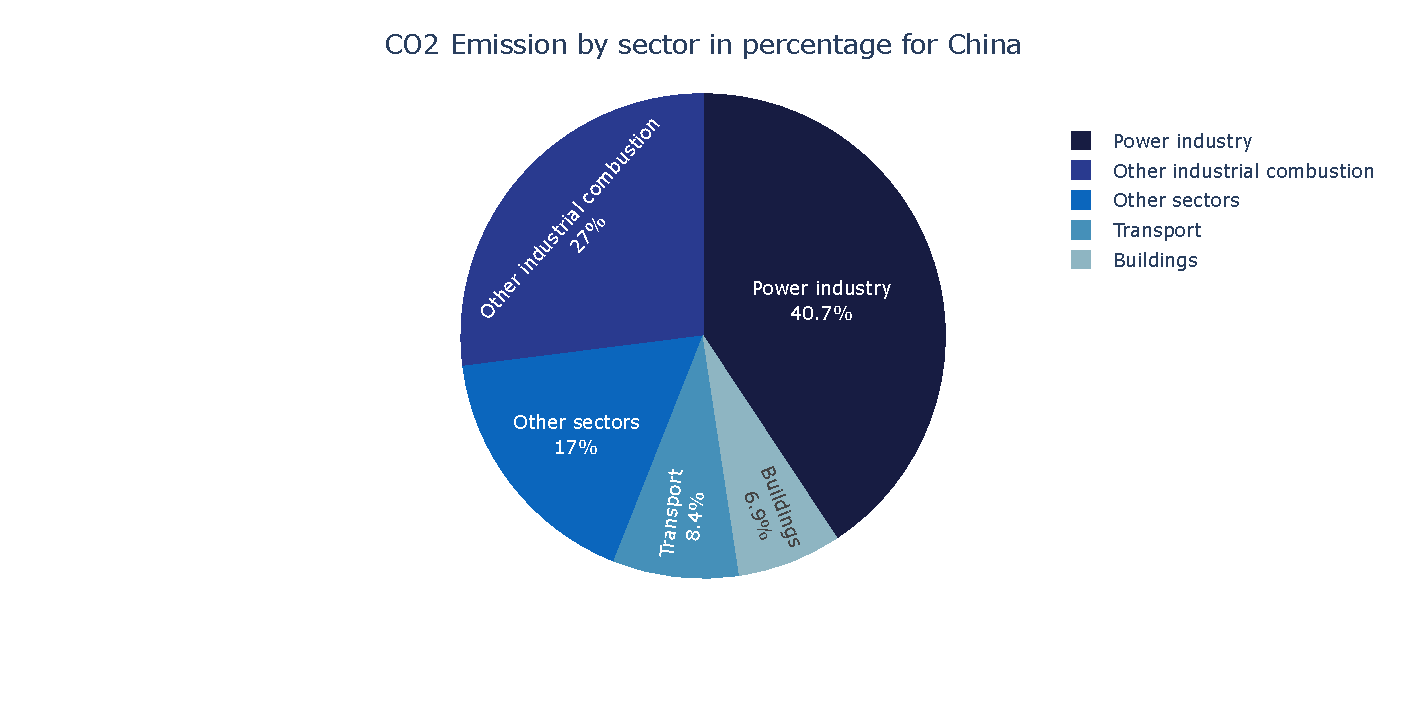
\includegraphics[width=0.45\linewidth]{../sector_overview/pie_plot_China}}\\
	\subfloat[EU]{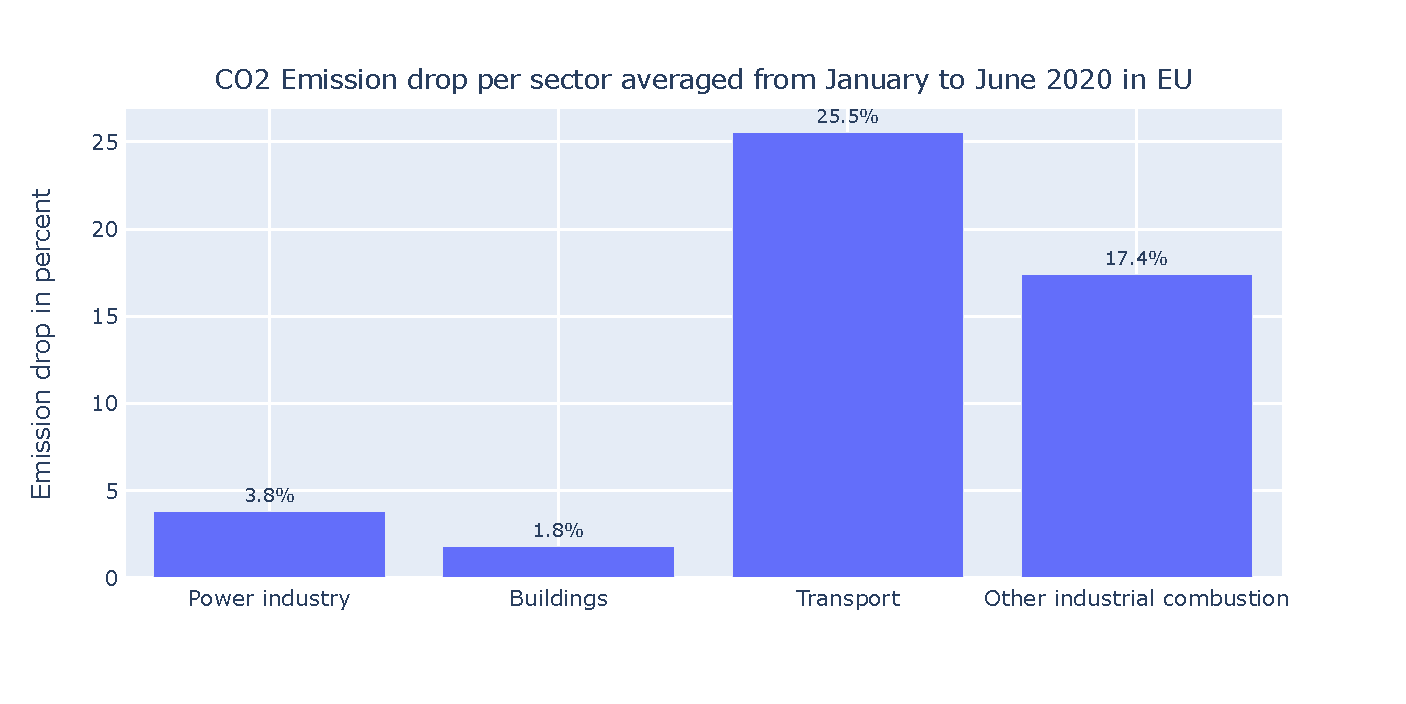
\includegraphics[width=0.45\linewidth]{../sector_overview/bar_plot_EU}}
	\subfloat[EU]{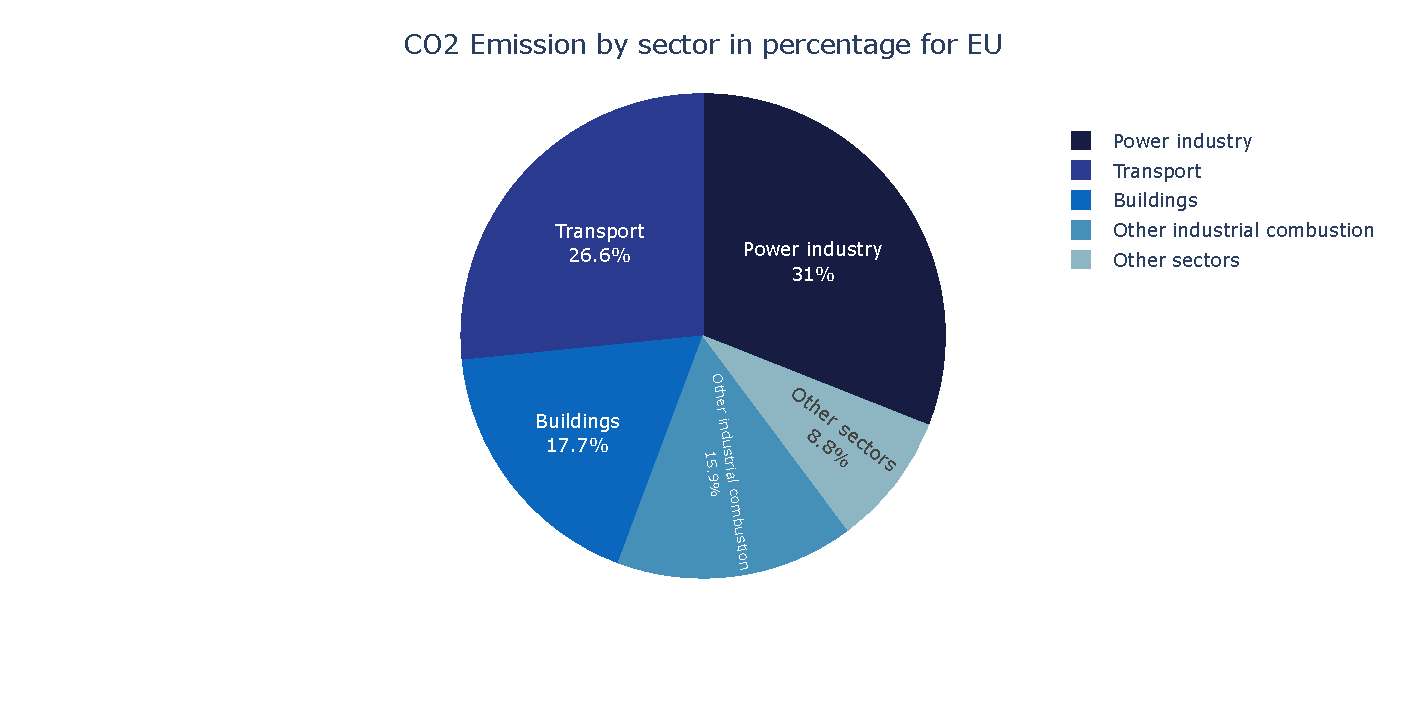
\includegraphics[width=0.45\linewidth]{../sector_overview/pie_plot_EU}}\\
	\caption{Averaged emission drop from January to June 2020 per country.}
	\label{fig:bar_plots}
\end{figure}

\begin{figure}[H]
	\centering
	\subfloat[India]{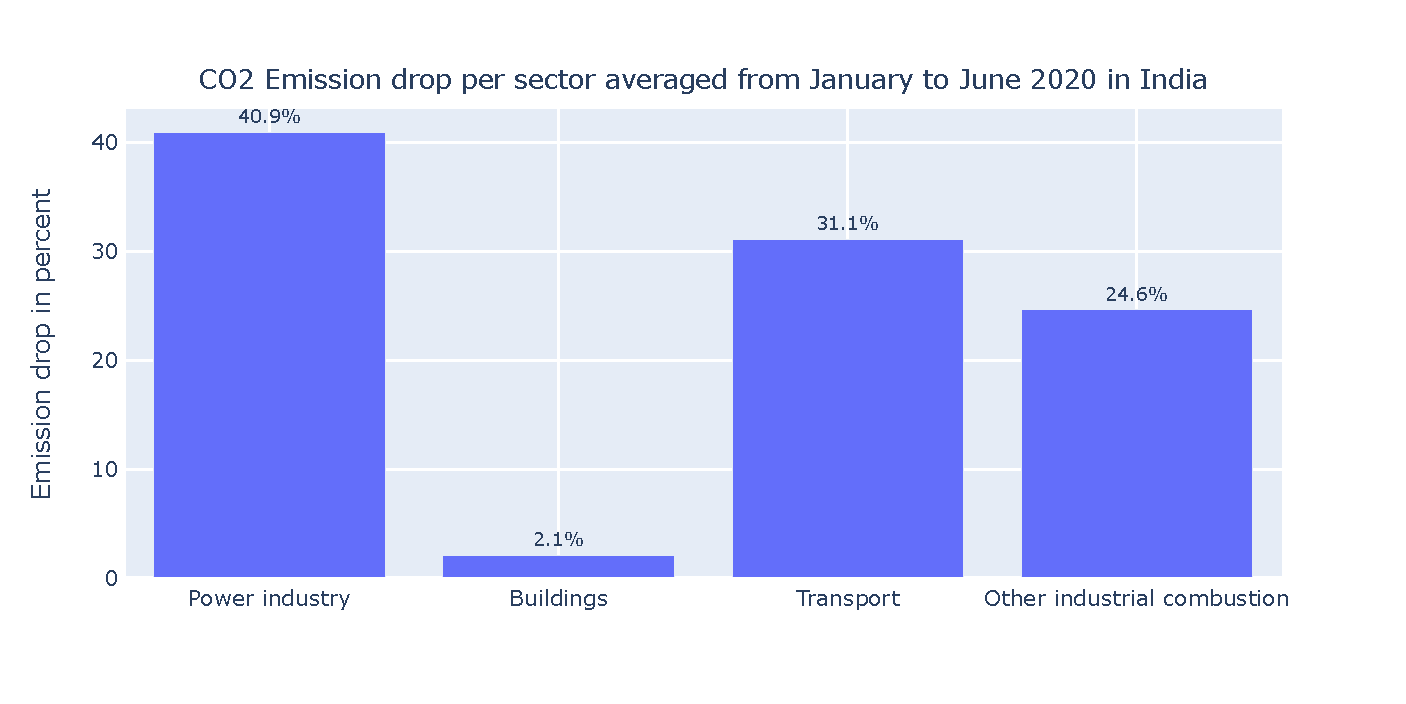
\includegraphics[width=0.45\linewidth]{../sector_overview/bar_plot_India}}
	\subfloat[India]{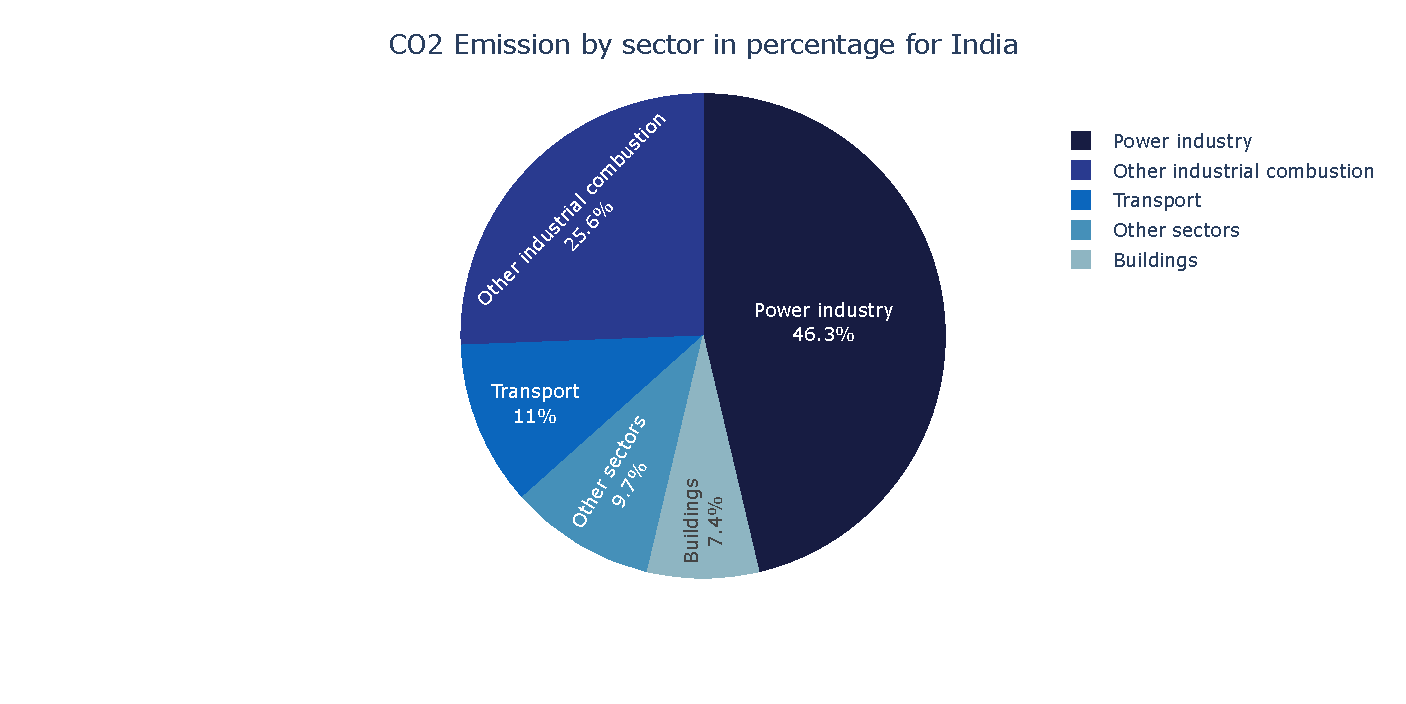
\includegraphics[width=0.45\linewidth]{../sector_overview/pie_plot_India}}\\
	\subfloat[Japan]{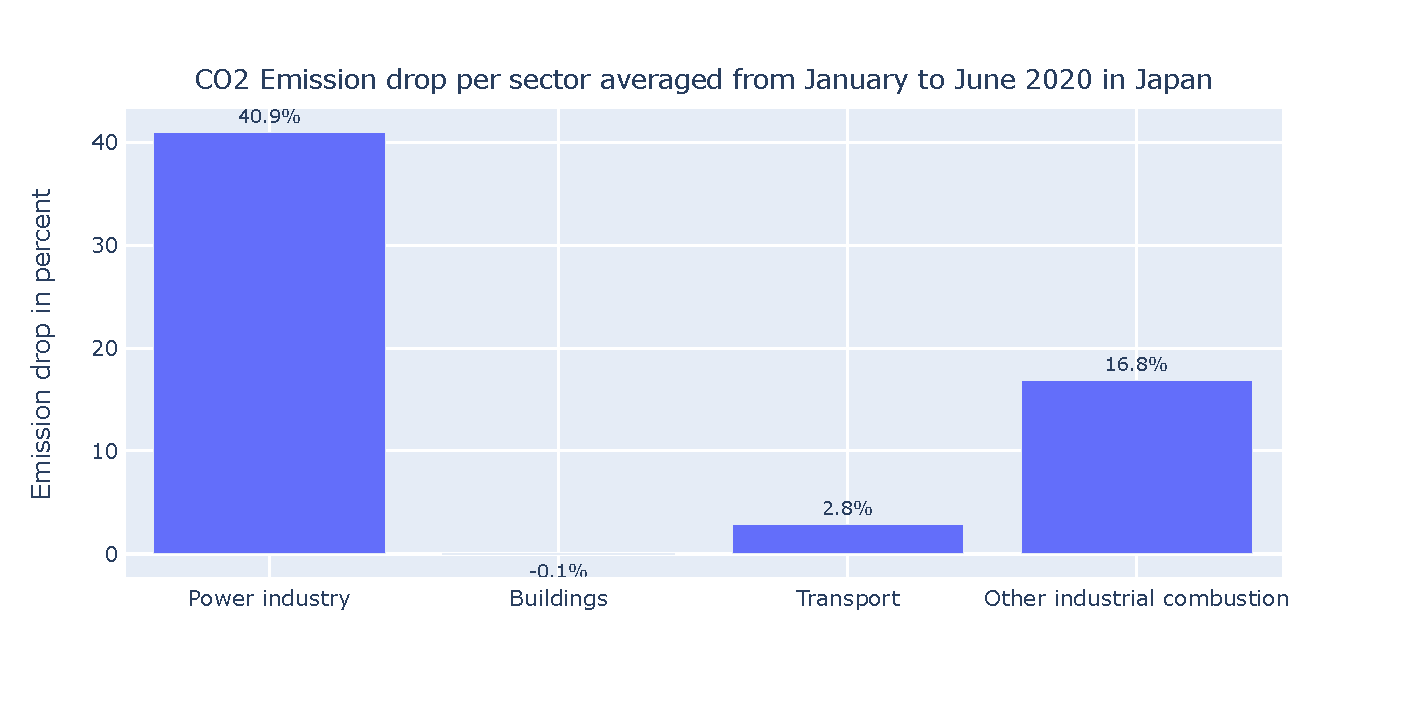
\includegraphics[width=0.45\linewidth]{../sector_overview/bar_plot_Japan}}
	\subfloat[Japan]{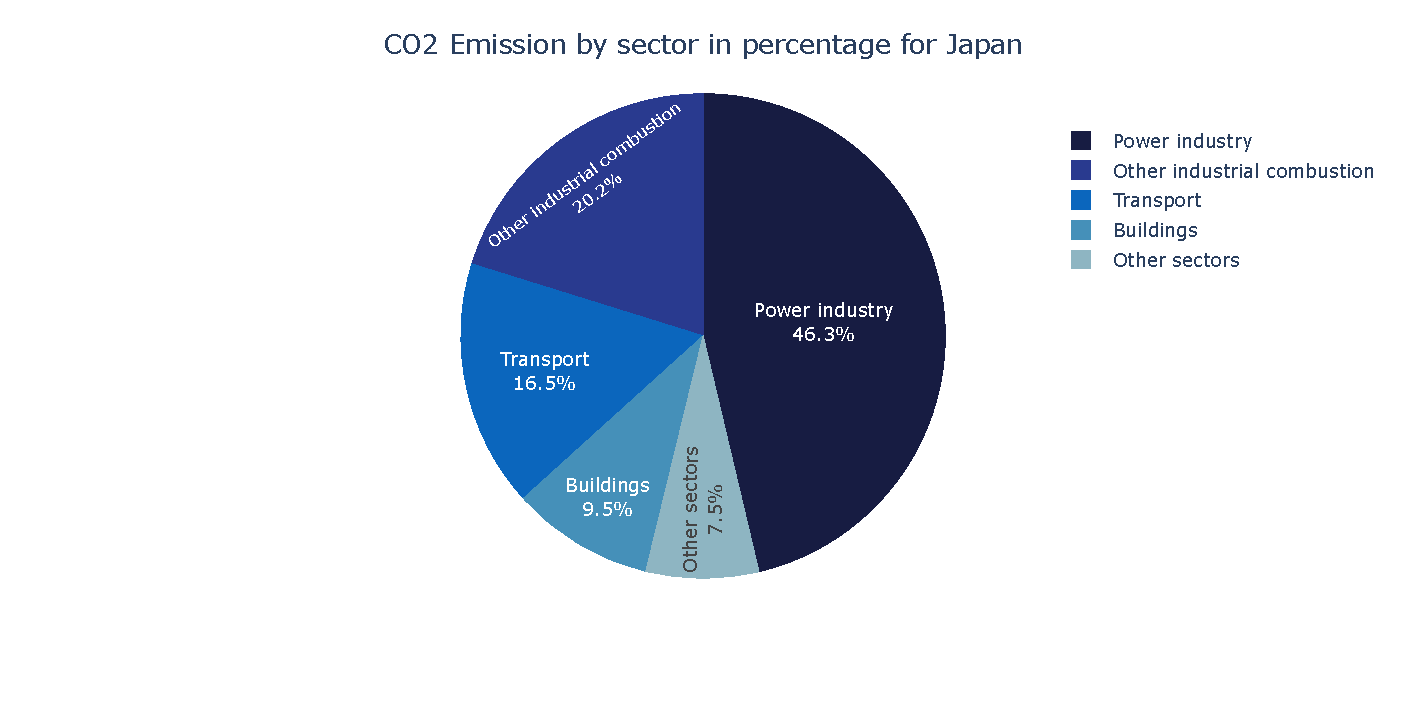
\includegraphics[width=0.45\linewidth]{../sector_overview/pie_plot_Japan}}\\
	\subfloat[Russia]{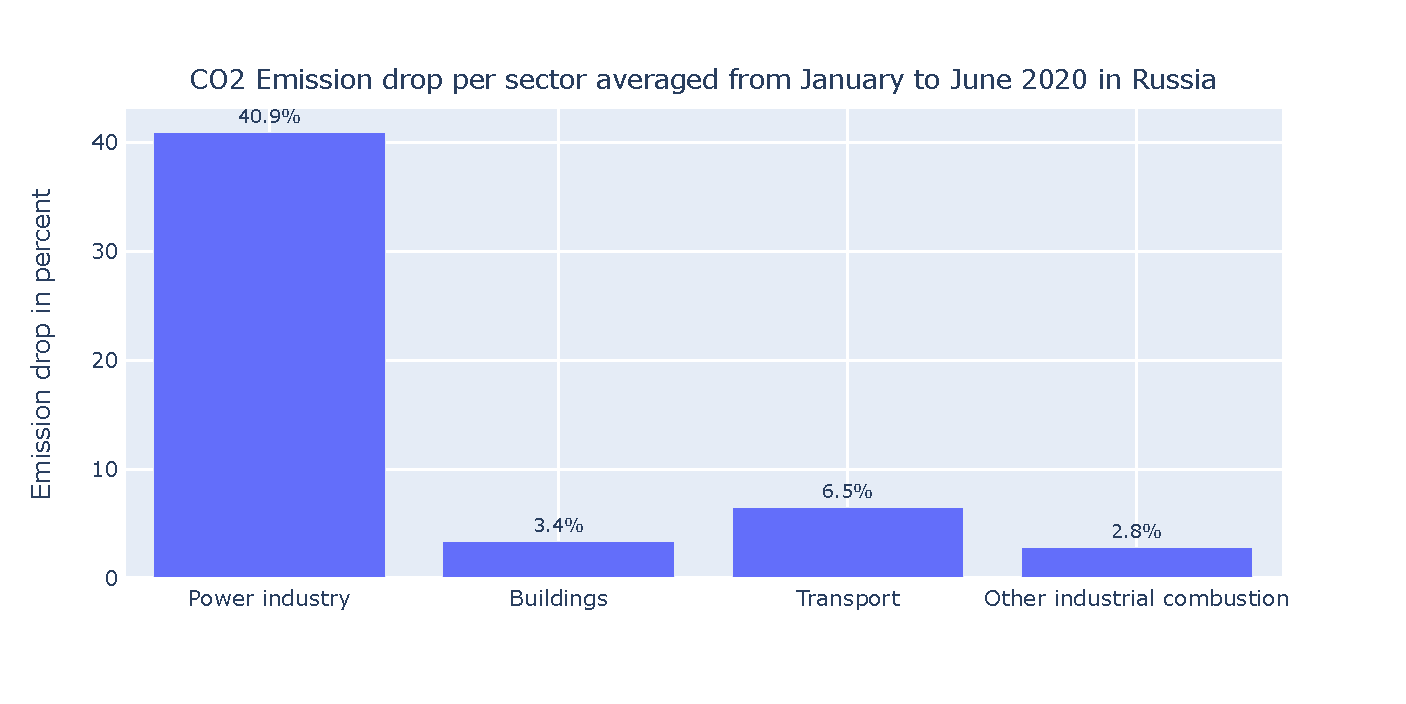
\includegraphics[width=0.45\linewidth]{../sector_overview/bar_plot_Russia}}
	\subfloat[Russia]{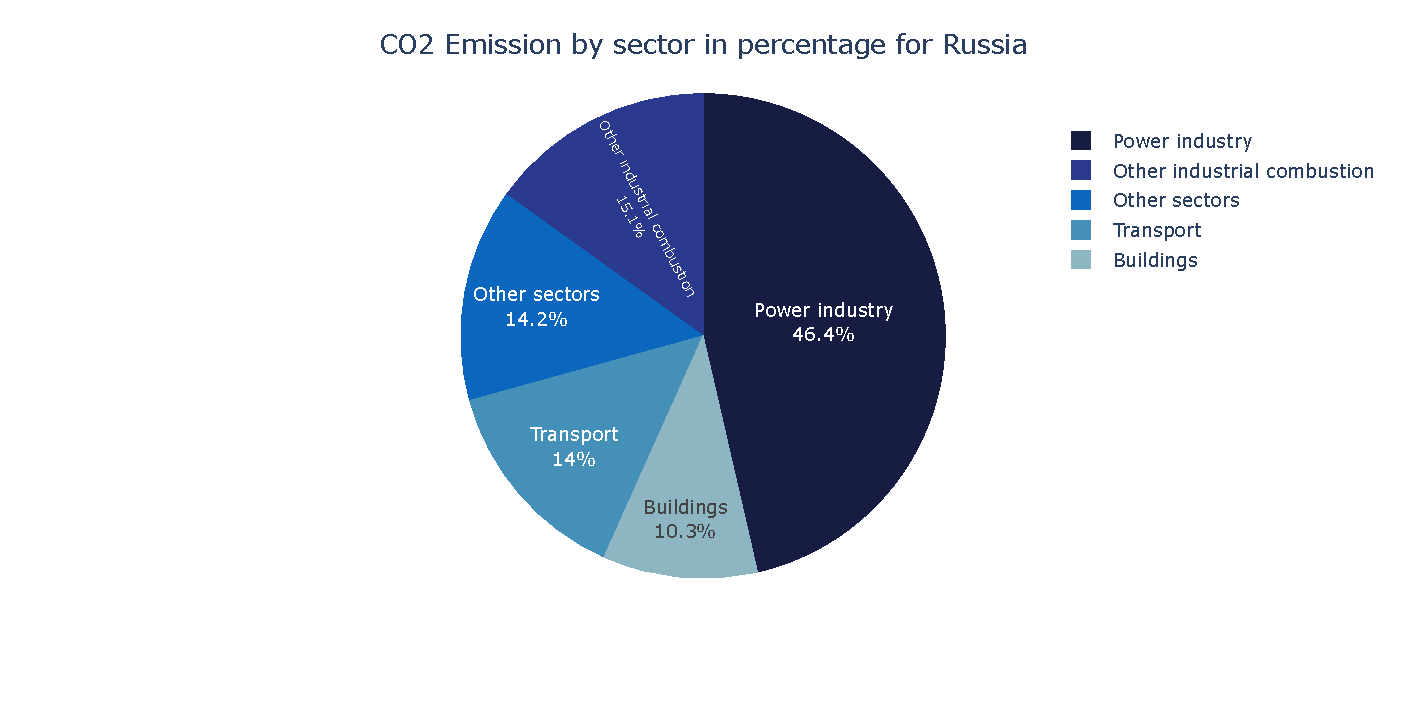
\includegraphics[width=0.45\linewidth]{../sector_overview/pie_plot_Russia}}\\
	\subfloat[United States]{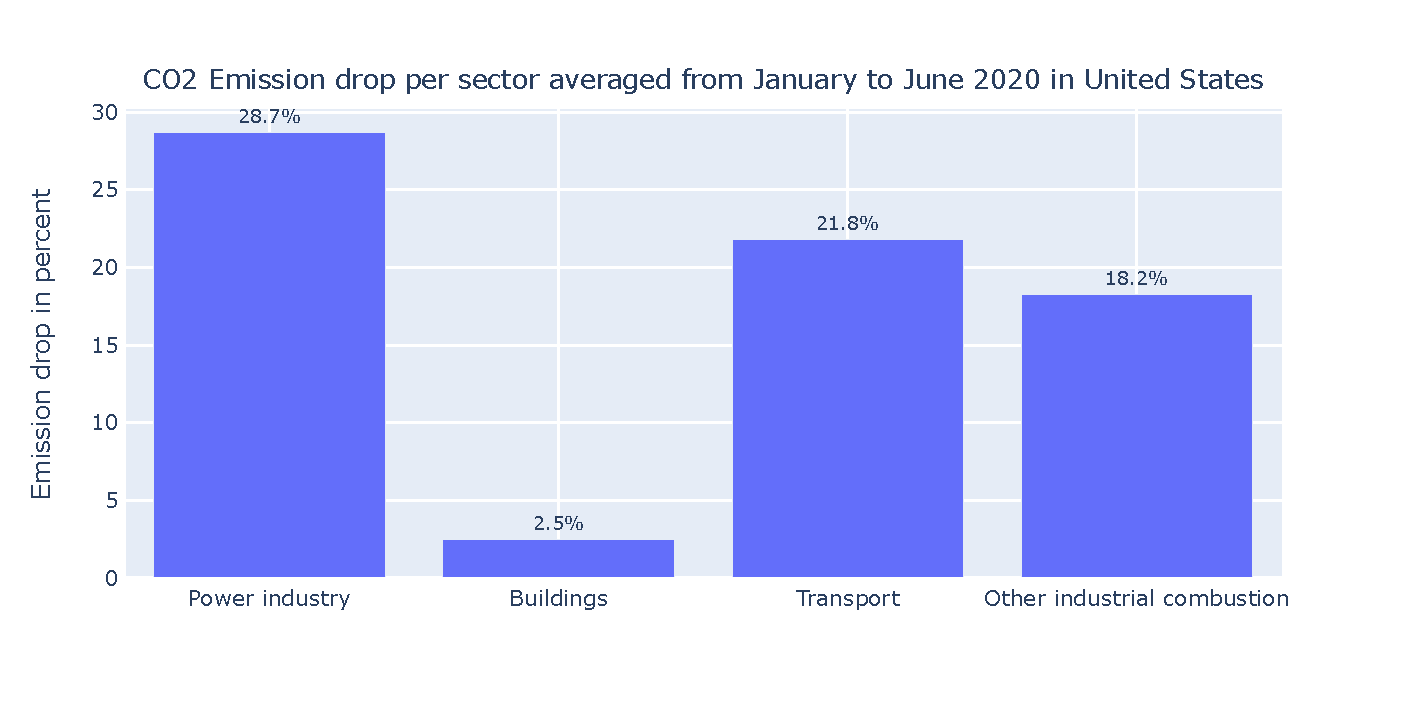
\includegraphics[width=0.45\linewidth]{../sector_overview/bar_plot_United_States}}
	\subfloat[United States]{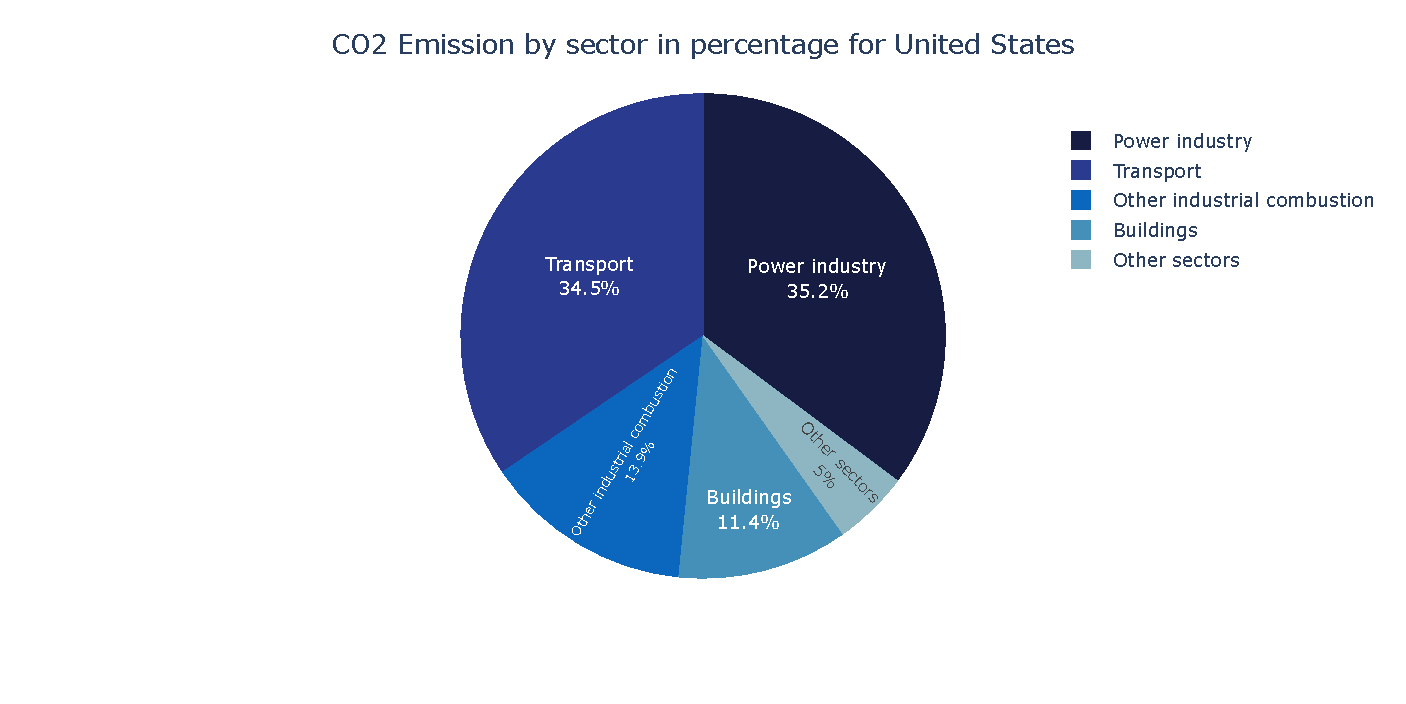
\includegraphics[width=0.45\linewidth]{../sector_overview/pie_plot_United_States}}
	\caption{Averaged emission drop from January to June 2020 per country.}
	\label{fig:bar_plots2}
\end{figure}

Even without inspection, one can easily identify the consistently most impacted sector to be the power industry of $20-40\%$. This sector includes fuel generation in general, which was in much less demand since February one could argue. The only region showing no significant decrease is the EU. This can be explained by the low fuel production in general, leading to a more stable profile.

The second sector of interest is the building sector. Here, remarkably low changes of $<5\%$ can be noted. In fact, one could conclude that the construction industry remained active during the pandemic. Also in Munich, we experienced a lot of construction activity for public projects like road improvements.

The third sector is the transport sector. We can note big decreases for Brazil, Canada, China, EU and the USA. 
Naturally, the travel activity in general is indicated by the performance of this sector. An explanation for Japan's low change in transport can be found, when we consider that Japan was among the last countries to start travel bans.
It remains unclear why Russia shows also less fluctuations.

The sector for other industrial combustions is connected to the production of goods. While China and Russia remained unaffected, all other countries in this analysis had a decent emission drop in this sector. China did a good job in confining the virus early, leading to less severe restrictions for the workforce in general. Russia's economy is more centered around fuel generation.

In conclusion, the biggest impact was the decrease of fuel production and transportation in general.



\subsection*{Largest COVID-19 impact for American and European continents}
\begin{figure}[H]
	\centering
	\subfloat[Cumulated cases per 100k inhabitants]{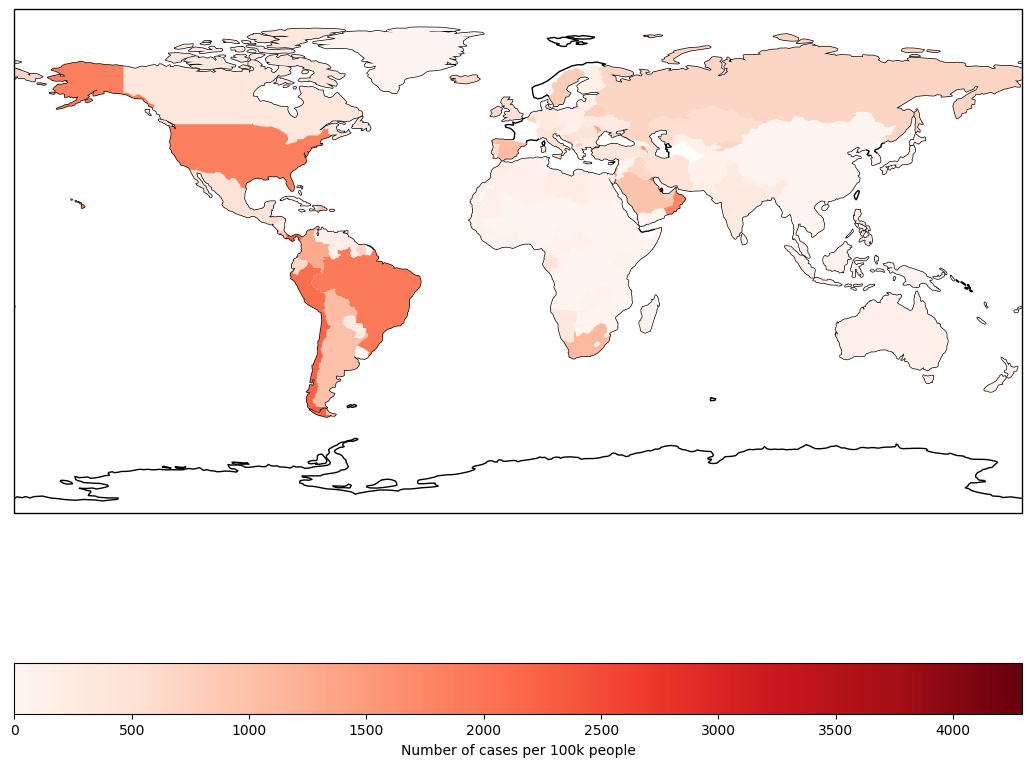
\includegraphics[width=0.5\textwidth]{../covid/case_rate.png}}
	\subfloat[Cumulated deaths per 100k inhabitants]{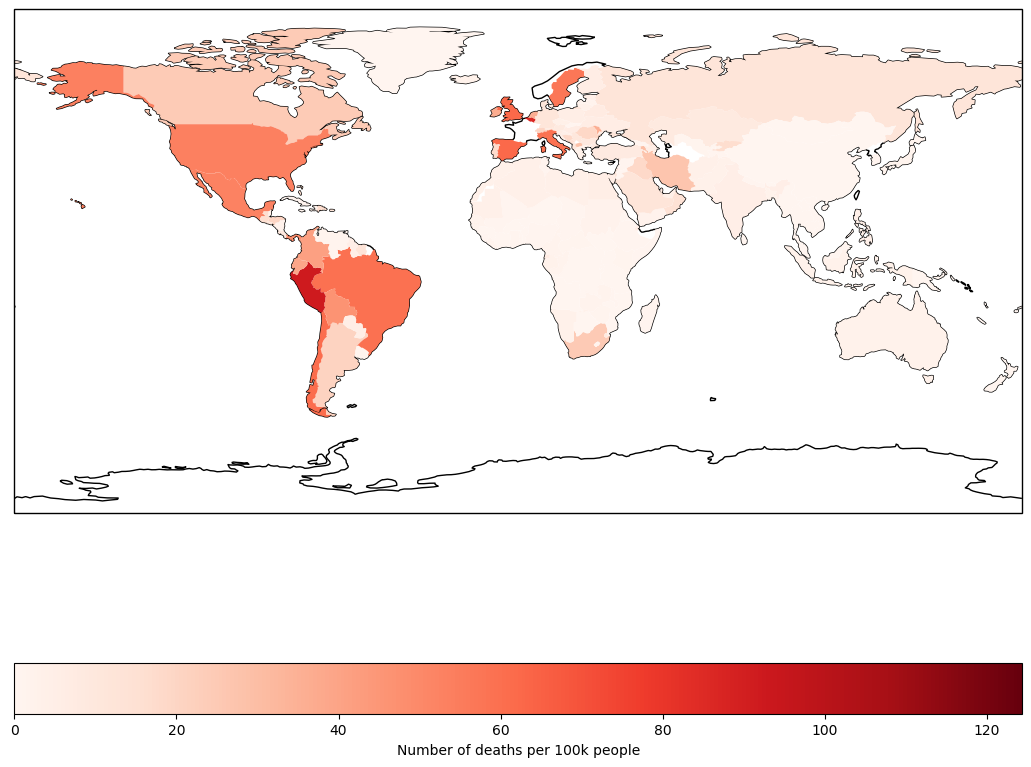
\includegraphics[width=0.5\textwidth]{../covid/death_rate.png}}
	\caption{COVID-19 impact visualization.}
	\label{fig:covid_cases}
\end{figure}% rate means per 100.000 inhabitants

As this report focuses on the impact of COVID-19 in \co emissions, we generated different maps to see the impact of COVID-19 all around the world. In combination with a dataset for the population in each country, we could normalize the cumulated deaths and cases by the population number to normalize the size of one country.

In Figure \ref{fig:covid_cases}, the case and death numbers per country are shown. Here, we can observe that the countries affected the most are the United States, Brazil and parts of the EU, which also are three of the eight countries that produce the most \co emissions. This reassures our choice of picking the eight biggest industries of the world, as we can hope for finding correlations.

\subsection*{No evidence with time series COVID-19 correlation}
In order to find a relation between the \co emissions and the COVID-19 data one can use the Pearson or the Spearman correlation between the predicted vectors from the different sectors and the death, active, and confirmed cases.

The correlation coefficient according to Pearson is sensitive to outliers. Therefore, we used the spearman method to identify the correlation coefficient.

\begin{figure}[h!]
	\centering
	\subfloat[COVID-19 data compared to the predicted overall vector for Japan]{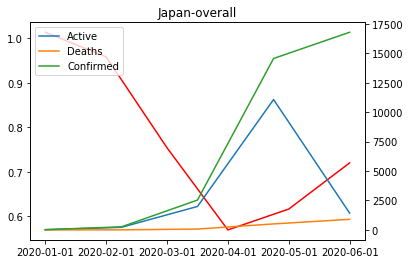
\includegraphics[width=0.5\linewidth]{ziedPNGS/japanOverall}}
	\subfloat[COVID-19 data compared to the predicted overall vector for EU]{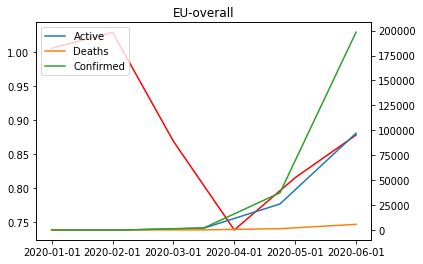
\includegraphics[width=0.5\linewidth]{ziedPNGS/euOverall}}
	\caption{Comparison between the predicted vectors and Covid-19 data.}
	\label{fig:Covid-predictedVectors}
\end{figure}

\begin{center}
\begin{table}[h!]
	\centering
	\begin{tabular}{llllll}
		\hline
		 Countries&Overall&buildings&mobility&power industry&other industries\\
		\hline
		\hline
		 Canada   & -0.6 & -0.6& -0.6& -0.999& -0.999\\
  		 China &  -0.199 & 0.7& -0.899& 0.099& -0.399\\
 		 Japan & -0.899 & 0.6& -0.999& -0.799& -0.7\\
 		 Russia &0.099 & -0.899& -0.099& -0.099& -0.799\\
  		 Brazil & -0.6 & 0.3& -0.6& -0.3& -0.7\\
		 India & -0.499& -0.899& -0.499& -0.099& -0.499\\
 		 United States & -0.714 & -0.028& -0.714& -0.428& -0.942\\
		 EU &-0.542 & -0.828& -0.542& -0.714& -0.714\\
		\hline &\\
	\end{tabular}
	\caption{Spearman correlation.}% linear
	\label{tab:spearman}	
\end{table}	
\end{center}

Even if the results show a negative correlation for some sectors activities and the CO2 emissions, only Japan's overall emissions seems to be affected by the increase of the COVID-19 cases.

A light tendency can be observed for the United States and the EU. By closer inspection in Figure \ref{fig:Covid-predictedVectors}, no strong relationship could be determined.

\subsection*{Nonlinear cumulated emission-COVID-19 correlation}

Therefore, we tried to correlate the integrated COVID-19 impact and the integrated emission drop. These correlations can be observed in Figure \ref{fig:emission_drop_over_normalized_deaths}. 

\begin{figure}[h!]
	\centering
	\subfloat[cases]{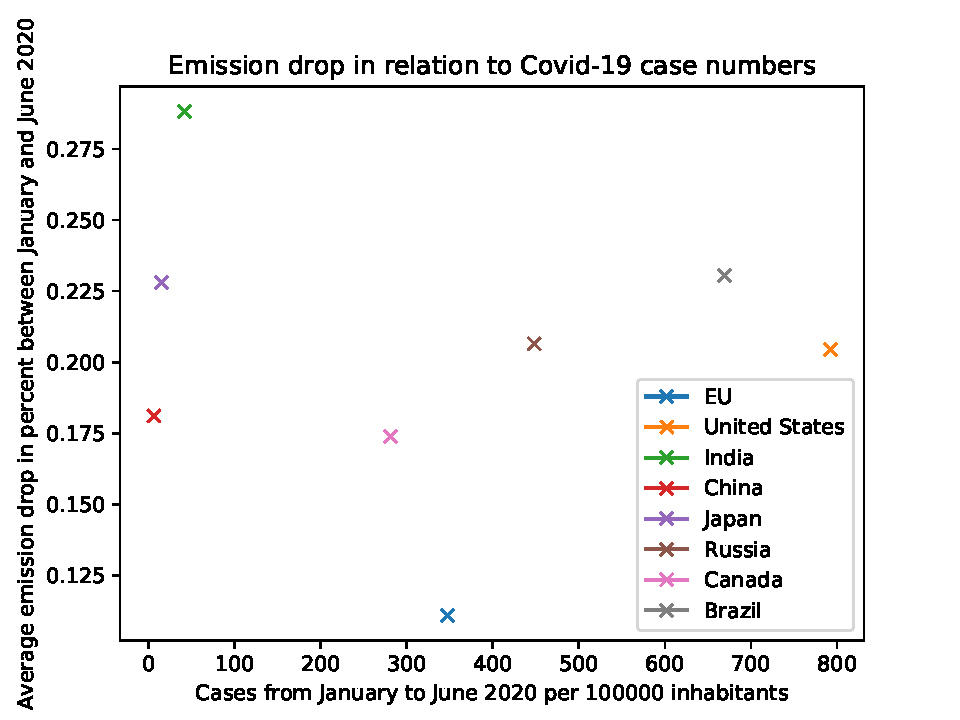
\includegraphics[width=0.5\linewidth]{../final_results/emission_drop_over_normalized_cases}}
	\subfloat[deaths]{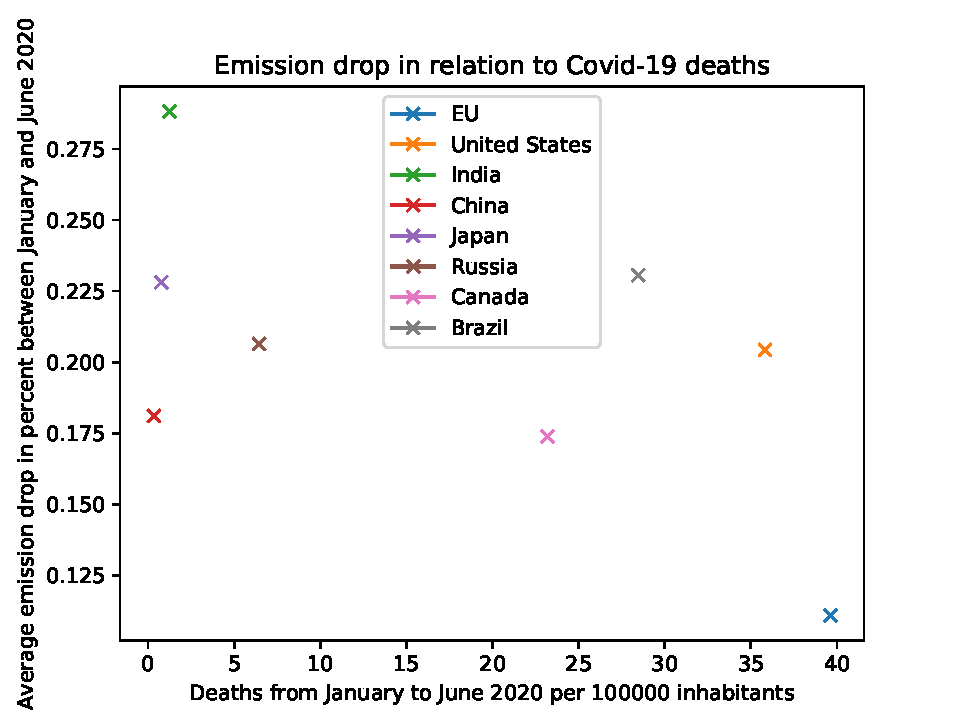
\includegraphics[width=0.5\linewidth]{../final_results/emission_drop_over_normalized_deaths}}
	\caption{Emission drop relation to COVID-19 case/death numbers.}
	\label{fig:emission_drop_over_normalized_deaths}
\end{figure}

In contrary to what we hoped, no linear trend could be extracted. Therefore, each country has to be evaluated independently. Two reasons could give rise to the noisiness: Either, there is no per country correlation, as the economies of different countries work differently and the complex net of globalization is not trivial to analyze, or our approach has significant weaknesses. Possibly, a combination of both makes this result plausible.

\subsection*{Relation to paris climate goals}

Even though no linear trend between COVID-19 cases and the \co emission drop could be seen in our analysis, one can still note the significant decrease in emissions during the corona crisis. In \autoref{fig:goals_lines}, the Paris climate goals of the biggest eight contributors are plotted in two ways. Subfigure (a) shows the reference year and the drop at the goal year, while Subfigure (b) normalizes the reference years to get a sense of the ambitiousness of each country.

\begin{figure}[H]
	\centering
	\subfloat[Compared to Referenced Year]{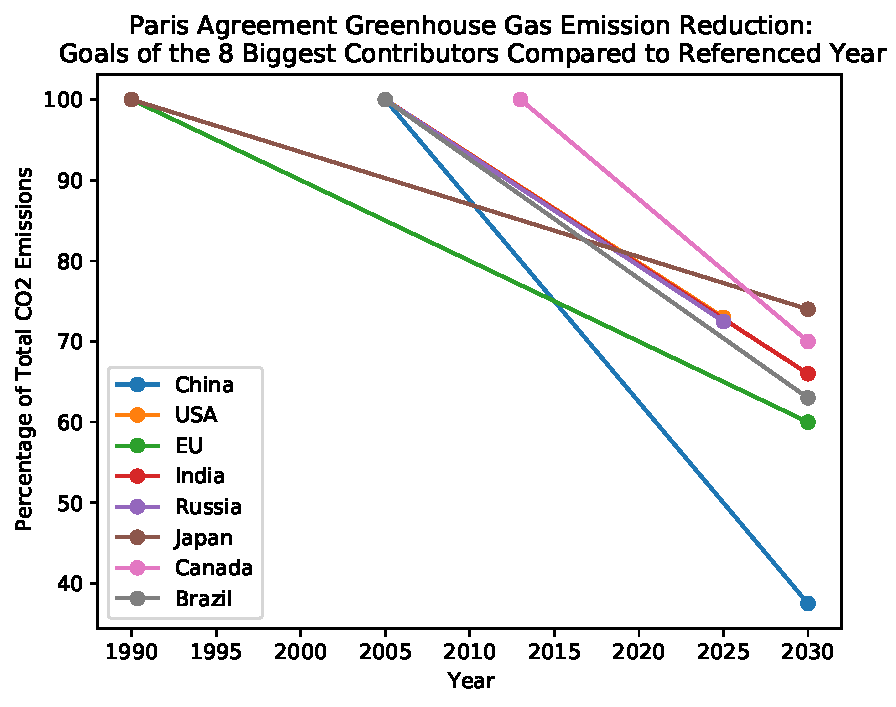
\includegraphics[width=0.5\textwidth]{img/co2goals_lines.pdf}}
	\subfloat[Compared to the 1.5°C Goal]{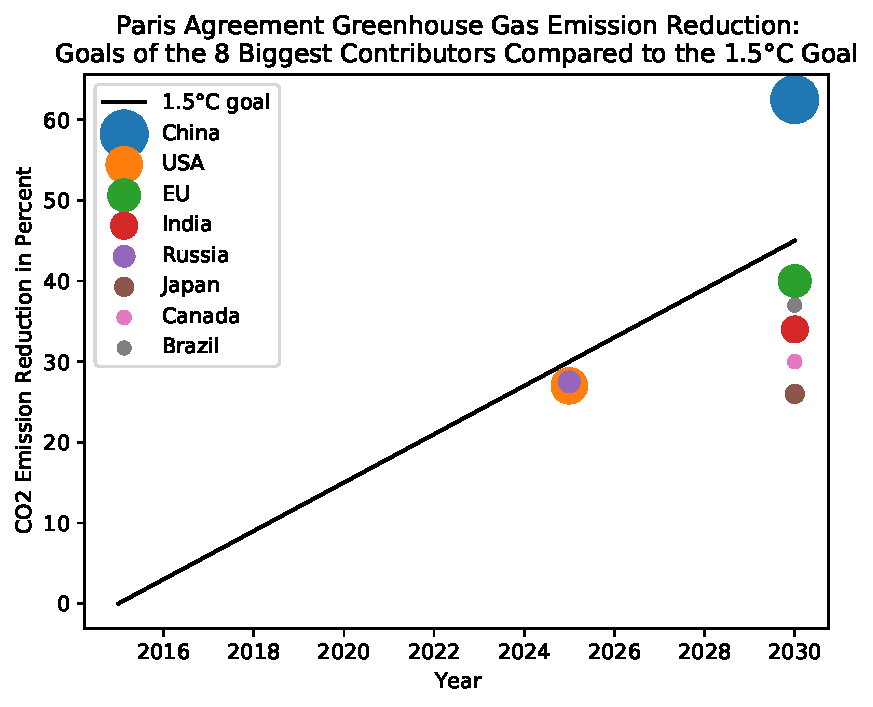
\includegraphics[width=0.5\textwidth]{img/co2goals_bubbles.pdf}}
	\caption{Goals of the 8 Biggest Contributors.}
	\label{fig:goals_lines}
\end{figure}

In conclusion, China has by far the most ambitious goals, which is even exceeding the requirements of the 1.5$^\circ C$ goal. Sadly, all of the other countries of interest are currently not even trying to achieve the 1.5$^\circ C$ goal in a treaty most countries are not even able to follow.

Comparing the emission drops from \autoref{fig:emission_drop_over_normalized_deaths} to the Paris agreement goals, one can observe an emission decrease of 20\% on average. This comes already very close to the emission drop range that is aimed for in the Paris agreement, but not quite.

The real challenge we are facing, is an emission reduction while all countries desperately try to grow their economy, mostly to the expense of mother nature.
